%Remember to include these in your preamble
\usepackage{tikz}
\tikzstyle{line} = [draw, -{Stealth[length=2mm, width=2mm]}, thick]

\newcommand{\weakness}{%
\begin{itemize}
    \item weakness1
    \item weakness2
    \item weakness3
    \item weakness4
\end{itemize}}

\newcommand{\strengths}{%
\begin{itemize}
    \item strength1
    \item strength2
    \item strength3
    \item strength4
\end{itemize}}

\newcommand{\opportunities}{%
\begin{itemize}
    \item opportunity1
    \item opportunity2
    \item opportunity3
    \item opportunity4
\end{itemize}}

\newcommand{\threats}{%
\begin{itemize}
    \item threat1
    \item threat2
    \item threat3
    \item threat4
\end{itemize}}

\begin{figure}[ht]
    \centering
    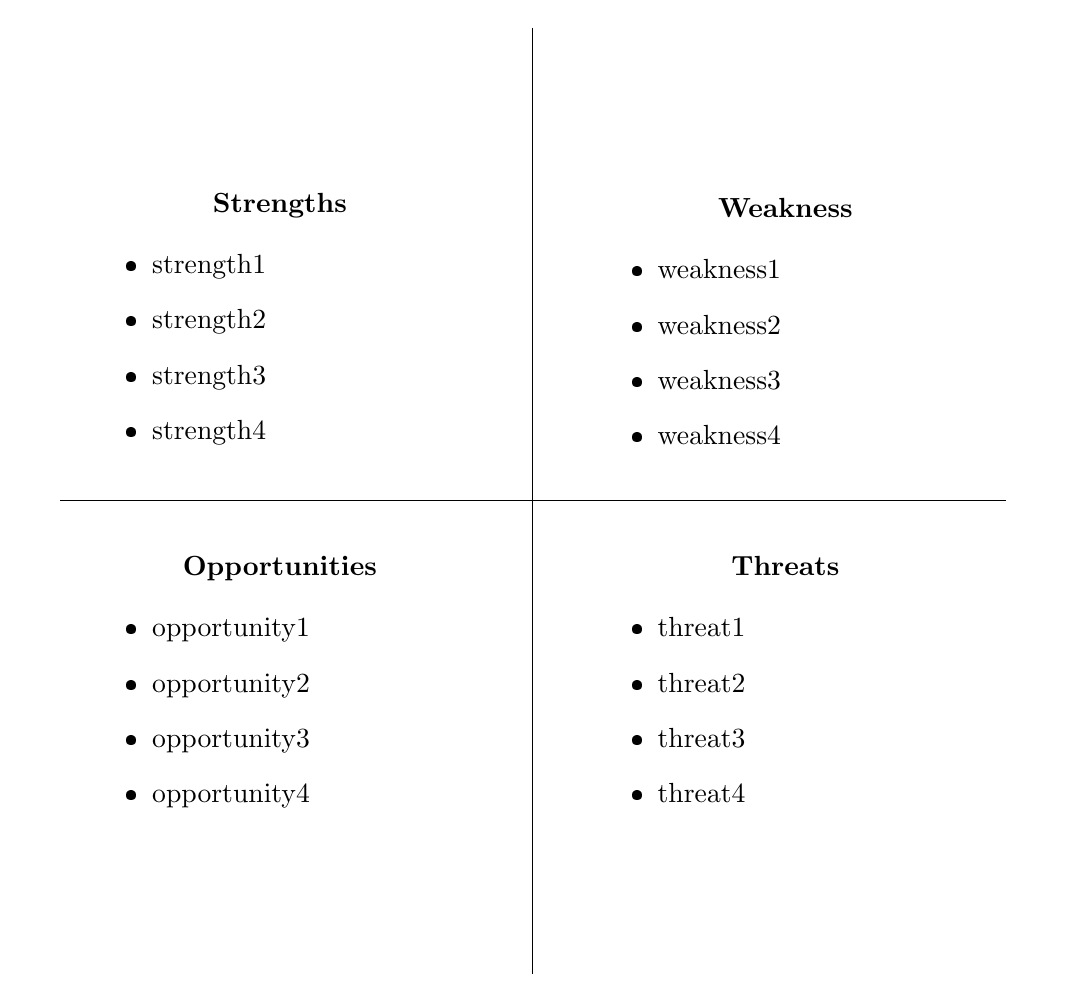
\begin{tikzpicture}
        \draw[line cap=rect] (-6,0) -- (6,0);
        \draw[line cap=rect] (0,-6) -- (0,6);
        
        \node[inner sep=20pt, anchor=south west, align=center, text width=5cm] (kvadrant1) at (0,0) {\textbf{Weakness}\\ \weakness};
        
        \node[inner sep=20pt, anchor=south east, align=center, text width=5cm] (kvadrant2) at (0,0) {\textbf{Strengths}\\ \strengths};
        
        \node[inner sep=20pt, anchor=north east, align=center, text width=5cm] (kvadrant3) at (0,0) {\textbf{Opportunities}\\ \opportunities};
        
        \node[inner sep=20pt, anchor=north west, align=center, text width=5cm] (kvadrant4) at (0,0) {\textbf{Threats}\\ \threats};
    \end{tikzpicture}%
    \caption{SWOT analysis}
    \label{fig_swot1}
\end{figure}
